\documentclass[12pt,twoside]{article}
\usepackage[a4paper,vmargin={30mm,30mm},hmargin={25mm,25mm}]{geometry}
\usepackage{amsmath}
\usepackage{amsfonts}
\usepackage{amssymb }
\usepackage{graphicx}
\usepackage{amsthm}
\usepackage[T1]{fontenc}
\usepackage{times}
\usepackage{lineno}
\usepackage{subfigure}
\usepackage{epstopdf}
\usepackage{bbm}
\usepackage{xcolor}
\usepackage[section]{placeins}
\renewcommand{\baselinestretch}{1.3} 



\begin{document}

\section{Generalized additive modeling approach}

\subsubsection*{Independent variables:}
\begin{itemize}
\item $X_1$ is patient age
\item $X_2$ is the probability a case has protective imprinting (estimated based on case birth year and country or origin).
\end{itemize}


\subsubsection*{Blocking variables (allow a different intercept for each level of each blocking variable):}
\begin{itemize}
\item $Z_1$ is vaccination in the past 12 months (0 = no, 1 = yes, 2 = unknown)
\item $Z_2$ is any antiviral use during treatment (0 = no, 1 = yes)
\item $Z_3$ is any underlying conditions (0 = no, 1 = yes)
\item $\mathbbm{1}_k$ is a binary indicator defining origin in country k.
\item $\mathbbm{1}_j$ is a binary indicator defining occurrence in season j. I assume the N. Hemisphere season spans Oct-March and the S. Hemisphere season spans April-Sept. Seasons include {NH.09-10, SH.10, NH.10-11, SH.11, ... SH.17}
\end{itemize}


\subsection*{General modeling approach}

\begin{equation}
f(x)= \alpha+g_1(X_1)+\beta_2X_2+\lambda_1Z_1+\lambda_2Z_2+\lambda_3Z_3+\sum_{k=1}^{n}c_k \mathbbm{1}_k +\sum_{j=1}^{m}s_j \mathbbm{1}_j
\end{equation}
\\Note: $g(X_1)$ is a natural spline on age, with a knot at age 65. The spline function fits one linear model to ages < 65, and one model to ages > 65. The two models are forced to join and become smooth and continuous at age = 65. The inclusion of this nonlinear relationship on age makes f(x) a generalized additive model, rather than a generalized linear model.\\ \\
I fit the above model to the following outcomes. For continuous outcome variables, equation 1 gives the overall model. For binary outcome variables, the model takes a logistic form:


\begin{equation}
p(x) = \frac{e^{f(x)}}{1 + e^{f(x)}}
\end{equation}
\\

\subsubsection*{Outcomes tested}

Note: Dataset 002 contains data collected from outpatients (patients enrolled with ILI, main outcome was confirmed influenza, although there is some questionable data on duration of infection here too). Dataset 003 contains data on hospitalized cases. Patients were only enrolled if hospitalized with confirmed influenza. Outcomes were infecting subtype, ICU admission, duraiton of symptoms, duration of hosptialization and death.

\begin{itemize}
\item \textbf{002: H1N1 incidence} Binary, 0 = no PCR confirmed influenza, 1 = confirmed H1N1, excluded all confirmed H3N2 and B cases, and excluded all unsubtyped cases.
\item \textbf{002: H3N2 incidence} Binary, 0 = no PCR confirmed influenza, 1 = confirmed H3N2, excluded all confirmed H1N1 and B cases, and excluded all unsubtyped cases.
\item \textbf{002: (Prolonged symptoms | confirmed H1N1) or (Prolonged symptoms | confirmed H3N2)} Binary outcome. Define prolonged symptoms as: symptoms lasting 10 days or more prior to study enrollment, or symptoms still present 14 days after study enrollment. (Weird definition, but this data is censored in weird ways. Honestly, given issues with the data I'm not sure if I trust this as a reliable outcome measure).
\item \textbf{003: (Symptom duration | confirmed H1N1) or (Symptom duration | confirmed H3N2)} Continuous outcome. The study only reports duration prior to enrollment. I asked about total duration, but apparently total duration is likely to measure duration of illness from secondary infections or complications after hospital admission. Again, not sure if this variable is a reliable measure of flu severity.
\item \textbf{002: (Hospital days | confirmed H1N1) or (Hospital days | confirmed H3N2)} Continuous outcome. Hospital days gives the number of days in the hospital after study enrollment. Total hospital days is also available, but many patients were hospitalized for conditions other than flu prior to study enrollment.
\item \textbf{002: (ICU | confirmed H1N1) or (ICU | confirmed H3N2)} Binary outcome.
\item \textbf{002: (Death | confirmed H1N1) or (Death | confirmed H3N2)} Binary outcome.
\end{itemize}


\subsection*{Constrained modeling approach}

A key challenge in this analysis is that probabilities of imprinting protection are intrinsically correlated with age. 

\begin{figure}
\centering
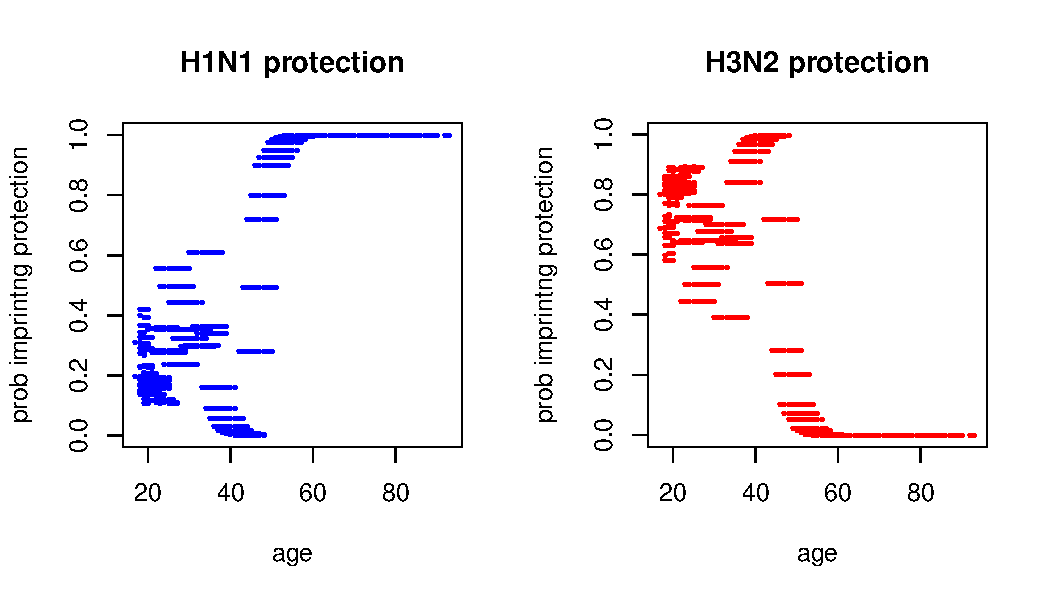
\includegraphics{correlation.pdf}
\caption{Age and probability of group1 or group 2 protection are correlated.}
\end{figure}

In an attempt to break this correlation and disentangle the effects of age and birth year, I fit a constrained model, which assumed a single relationship between age and outcome for both infecting subtypes. In other words, I assumed age would have the same effects on outcomes caused by H1N1 and H3N2 infection, rather than allowing unique effects for each subtype.

The constrained age curve captures age-specific epidemiological patterns independent of the challenge subtype, such as age-specific differences in social mixing, in health care seeking behavior, and in immune competence. Constrained age effects will not capture differences in age-specific histories of influenza exposure, which may be subtype specific.

I also assumed the effects of antiviral treatment, underlying symptoms and country would be the same, regardless of whether infection was caused by H1N1 or H3N2 and constrained these relationships to take the same form for H1N1 and H3N2 outcomes.

Finally, after detecting no significant interaction between subtype and probability of imprinting protection, I also fit a single relationship between probability of imprinting protection and outcome.

I did consider interactions between season and subtype (because different subtypes dominate circulation in different seasons), and included a three-way interaction between vaccination status, season and subtype (because vaccine efficacy is subtype-specific and changes from season to season).


\end{document}